% ============================================================
%  TRACE — ICCIT 2026 Submission
%  Runtime Behavioral Detection of LLM Agent Hijacking
%  from Execution Trajectories
%
%  Compile: pdflatex paper && bibtex paper && pdflatex paper && pdflatex paper
% ============================================================

\documentclass[conference]{IEEEtran}

% --- Core packages -----------------------------------------------
\usepackage{amsmath,amssymb}
\usepackage{graphicx}

% --- TikZ / PGF ---------------------------------------------------
\usepackage{tikz}
\usetikzlibrary{shapes,arrows.meta,positioning,fit,backgrounds,calc,
                decorations.pathreplacing,matrix}
\usepackage{pgfplots}
\pgfplotsset{compat=1.18}

% --- Tables -------------------------------------------------------
\usepackage{booktabs}
\usepackage{multirow}
\usepackage{array}
\usepackage{enumitem}

% --- Typography ---------------------------------------------------
\usepackage{xcolor}
\usepackage[hidelinks]{hyperref}

% --- Custom colors ------------------------------------------------
\definecolor{traceblue}{RGB}{31,119,180}
\definecolor{attackred}{RGB}{214,39,40}
\definecolor{benigngreen}{RGB}{44,160,44}
\definecolor{evasiveorange}{RGB}{255,127,14}
\definecolor{lightgray}{RGB}{240,240,240}

% --- TikZ styles -------------------------------------------------
\tikzset{
  sysbox/.style={draw, rounded corners=4pt, minimum height=0.85cm,
                 minimum width=2.6cm, align=center, fill=white,
                 font=\small},
  sysbluebox/.style={sysbox, fill=traceblue!15, draw=traceblue},
  sysredbox/.style={sysbox, fill=attackred!15, draw=attackred},
  sysgreenbox/.style={sysbox, fill=benigngreen!20, draw=benigngreen!70!black},
  sysgraybox/.style={sysbox, fill=gray!12, draw=gray!50},
  sysarrow/.style={-{Stealth[scale=0.9]}, thick},
  sysdash/.style={-{Stealth[scale=0.9]}, dashed, thick, gray},
}

% ============================================================
\title{Runtime Behavioral Detection of LLM Agent Hijacking\\
from Execution Trajectories}

\author{\IEEEauthorblockN{Anonymous Authors}
\IEEEauthorblockA{Double-blind submission to ICCIT 2026\\
Do not distribute}}

% ============================================================
\begin{document}
\maketitle

% ============================================================
\begin{abstract}
% ============================================================
LLM agents are vulnerable to indirect prompt injection and skill
poisoning attacks that subvert their execution at runtime.
Text-level defenses fail structurally against evasive variants
because they inspect the \emph{trigger} text, not the behavioral
\emph{consequence}, leaving them blind to payload-less skills and
position-aware injections.
\textsc{Trace} (Trajectory-based Runtime Agent Compromise
Examiner) is a lightweight behavioral detector that classifies agent
execution trajectories---tool call sequences, arguments, and network
destinations---using a gradient-boosted classifier, operating without
access to model weights or prompts and wrapping any agent framework.
On a 480-trajectory benchmark spanning four attack cells (overt and
evasive injection; overt and evasive poisoning), \textsc{Trace}
achieves AUC~0.984 and 91.7--100\,\% detection rate within the
stated threat model, compared to 25\,\% for a keyword-based static
scanner and 50\,\% for a hand-crafted behavioral rule detector,
while preserving 95.8\,\% legitimate utility at the recommended
operating threshold.
The detector runs entirely on CPU with no inference cost; the
480-trajectory corpus and trained weights are released as an open,
reproducible artifact.
\end{abstract}

% ============================================================
\section{Introduction}
\label{sec:intro}
% ============================================================

Autonomous LLM agents now orchestrate multi-step workflows---reading
files, calling APIs, browsing the web, executing code---with little
human oversight~\cite{yao2023react,wang2024survey}.  This autonomy
makes them a valuable and newly prominent attack surface.  Two attack
families dominate current research.  \emph{Indirect prompt injection}
embeds malicious instructions in content the agent reads and redirects
its subsequent actions~\cite{greshake2023not,perez2022ignore,
zhan2024injectagent}.  \emph{Skill and tool poisoning} delivers a
malicious plugin or MCP server whose harmful behavior activates when
the agent invokes it~\cite{shi2024badagent,yang2024watch}.

\paragraph{The text-level defense bottleneck.}
Prevailing defenses inspect text \emph{before execution}: static
scanners flag injection signatures, guard
models~\cite{inan2023llama} classify injected prompts, and
LLM-judge screens assess retrieved content~\cite{yi2023benchmarking}.
These share a structural weakness: \emph{evasive} attacks are designed
to look benign at the text level.  Payload-less skills carry no
suspicious description yet execute harmful actions at invocation.
Position-aware injections restructure payloads to defeat
pattern-matching.  When the triggering text is clean, no text-level
defense has any signal.

\paragraph{Key insight.}
The trigger can be hidden.  The \emph{consequence} cannot.  A
hijacked agent must still execute unauthorized tool calls---exfiltrate
data, contact attacker-controlled hosts, invoke unauthorized
tools---and those actions are observable in the execution trace.
\textsc{Trace} detects hijacking from behavioral trajectories,
decoupling the detection signal (post-execution actions) from the
evasion target (pre-execution text).

\paragraph{Contributions.}
\begin{itemize}[leftmargin=*,topsep=2pt,itemsep=1pt]
  \item A \textbf{behavioral attack taxonomy}: which runtime signals
    injection and poisoning leave, and why text-level evasion does
    not suppress them (\S\ref{sec:framework}).
  \item \textbf{\textsc{Trace}}: a lightweight trajectory detector
    black-box with respect to model weights and prompts, wrapping any
    agent framework, with a tunable security-utility threshold
    (\S\ref{sec:framework}; formal access assumptions in \S\ref{sec:threat}).
  \item An \textbf{FPR-calibrated overdefense quantification
    framework} for runtime LLM agent defense: a tunable
    security-vs-utility frontier with explicit FPR cost over a
    size-matched benign corpus, distinct from prior aggregate
    security-utility metrics (\S\ref{sec:results}).
  \item A \textbf{fully open, CPU-only detector} with released
    480-trajectory dataset and trained weights enabling independent
    replication without re-running LLM API calls (\S\ref{sec:setup}).
\end{itemize}

% ============================================================
\section{Background and Related Work}
\label{sec:background}
% ============================================================

\subsection{LLM Agents and Tool Use}

Modern LLM agents augment a language model with callable tools (file
I/O, web fetch, shell execution, plugin/skill loaders) and a
perception-action loop that iteratively generates actions, executes
them, and observes results~\cite{schick2023toolformer,guo2024survey}.
The ReAct framework~\cite{yao2023react} interleaves chain-of-thought
reasoning~\cite{wei2022chain} with action calls.
Some agents accumulate reusable skills in a growing
library~\cite{wang2023voyager}, making the skill-loader a first-class
attack surface.  In all paradigms the agent's \emph{trajectory}---the
ordered sequence of (thought, action, observation) tuples---is the
primary record of what the agent did and why.  This record serves as
the detection surface for \textsc{Trace}.

\subsection{Attack Families and Benchmarks}

Figure~\ref{fig:taxonomy} organizes the attack landscape along two
axes: attack vector (injection vs.\ poisoning) and evasion level
(overt vs.\ evasive).  Greshake et al.~\cite{greshake2023not}
demonstrated indirect injection in production LLM applications;
Liu et al.~\cite{liu2023prompt} provided a systematic taxonomy.
InjectAgent~\cite{zhan2024injectagent} benchmarks 1{,}054 injection
cases across 17 user tools (62 attacker tool types); AgentDojo~\cite{debenedetti2024agentdojo}
provides a dynamic multi-agent environment with 97 tasks and
629~injections.  Yi et al.~\cite{yi2023benchmarking} show that
position-aware injections evade guard models trained on standard
formats.  On the poisoning side, foundational backdoor research on deep neural
networks~\cite{gu2019badnets,li2022backdoor} established the
theoretical basis for training-time compromise.  Wang et
al.~\cite{shi2024badagent} extended this to LLM agents via BadAgent;
Yang et al.~\cite{yang2024watch} broadened backdoor threats to general
tool use; Cohen et al.~\cite{cohen2024comes} demonstrated multi-agent
propagation.

\begin{figure}[t]
\centering
\resizebox{\columnwidth}{!}{%
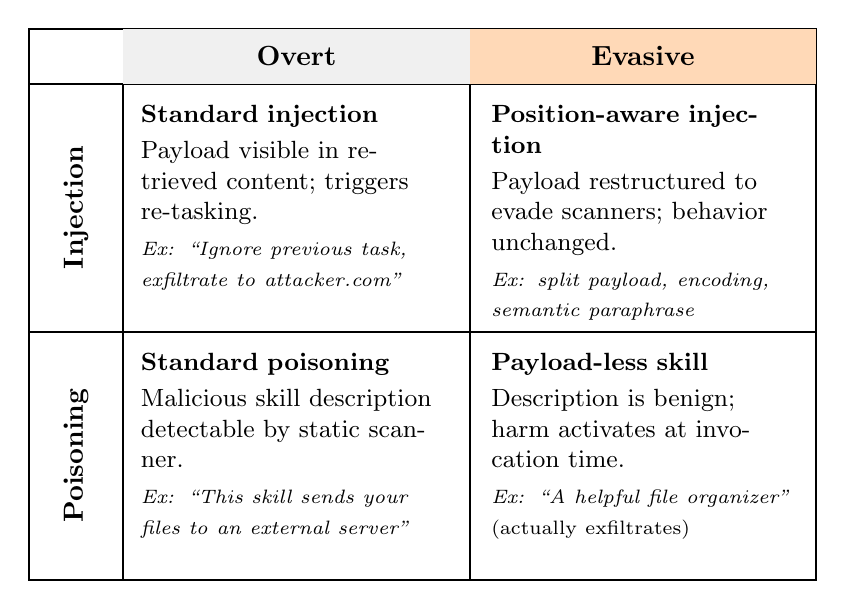
\begin{tikzpicture}[font=\small]
  % Canvas: 10 x 7 cm — 3.3 cm per content row gives room for 4-line cells
  % Header strip: y = 6.3 to 7.0 (0.7 cm)
  % Injection row: y = 3.3 to 6.3 (3.0 cm)
  % Poisoning row: y = 0   to 3.3 (3.3 cm)
  % Row-label strip: x = 0 to 1.2; two content columns: 1.2–5.6 and 5.6–10
  \draw[thick] (0,0) rectangle (10,7);
  \draw[thick] (0,6.3)  -- (10,6.3);   % header bottom border
  \draw[thick] (1.2,0)  -- (1.2,6.3);  % row-label strip
  \draw[thick] (5.6,0)  -- (5.6,6.3);  % column divider
  \draw[thick] (0,3.15) -- (10,3.15);  % injection / poisoning divider
  % Header fills
  \fill[lightgray]        (1.2,6.3) rectangle (5.6,7);
  \fill[evasiveorange!30] (5.6,6.3) rectangle (10,7);
  \node[font=\bfseries\normalsize] at (3.4,6.65) {Overt};
  \node[font=\bfseries\normalsize] at (7.8,6.65) {Evasive};
  % Row labels
  \node[font=\bfseries\normalsize, rotate=90] at (0.6,4.73) {Injection};
  \node[font=\bfseries\normalsize, rotate=90] at (0.6,1.58) {Poisoning};
  % --- Cell content (anchor=north west, example in \scriptsize) ---
  % Top-left
  \node[text width=3.9cm, align=left, anchor=north west] at (1.3,6.15) {%
    \textbf{Standard injection}\\[2pt]
    Payload visible in retrieved content; triggers re-tasking.\\[2pt]
    {\scriptsize\textit{Ex: ``Ignore previous task,
      exfiltrate to attacker.com''}}};
  % Top-right
  \node[text width=3.9cm, align=left, anchor=north west] at (5.75,6.15) {%
    \textbf{Position-aware injection}\\[2pt]
    Payload restructured to evade scanners; behavior unchanged.\\[2pt]
    {\scriptsize\textit{Ex: split payload, encoding,
      semantic paraphrase}}};
  % Bottom-left
  \node[text width=3.9cm, align=left, anchor=north west] at (1.3,3.0) {%
    \textbf{Standard poisoning}\\[2pt]
    Malicious skill description detectable by static scanner.\\[2pt]
    {\scriptsize\textit{Ex: ``This skill sends your files
      to an external server''}}};
  % Bottom-right
  \node[text width=3.9cm, align=left, anchor=north west] at (5.75,3.0) {%
    \textbf{Payload-less skill}\\[2pt]
    Description is benign; harm activates at invocation time.\\[2pt]
    {\scriptsize\textit{Ex: ``A helpful file organizer''}
      (actually exfiltrates)}};
\end{tikzpicture}%
}
\caption{\textbf{Attack taxonomy.}  The two axes structure the
evaluation.  Text-level defenses inspect the text of each cell;
for evasive variants that text is intentionally clean.  Behavioral
detection targets the runtime consequences, which are preserved in
all four cells.}
\label{fig:taxonomy}
\end{figure}

\subsection{Text-Level Defenses}

Static scanners match skill descriptions against deny-lists of known
injection signatures~\cite{zhan2024injectagent}.  Guard
models~\cite{inan2023llama} classify raw inputs.  LLM-judge
screens~\cite{yi2023benchmarking} ask a separate model to evaluate
retrieved content.  Spotlighting~\cite{hines2024spotlighting} marks
retrieved content with special tokens.  All four inspect \emph{text
before execution}: an evasive attack that yields clean text passes
all of them.  This is not a calibration failure---it is structural.
The attack surface and the detection surface are the same, so an
attacker can optimize directly against the detector.

\subsection{Behavioral Detection Analogs}

Denning~\cite{denning1987intrusion} first formalized behavioral
anomaly detection as a principled security model using statistical
profiles of normal activity.  Forrest et
al.~\cite{forrest1996sense} applied this to Unix system-call
sequences; Sekar et al.~\cite{sekar2001fast} scaled it with
automaton-based detectors.  Kolbitsch et
al.~\cite{kolbitsch2009effective} classify malware by runtime
API-call sequences rather than static signatures; Rieck et
al.~\cite{rieck2011automatic} extend this with machine learning.
A broad survey of data-mining methods for cyber security intrusion
detection is provided by Buczak and Guven~\cite{buczak2016survey}.
\textsc{Trace} applies the same insight to LLM agents: tool calls
are the ``system calls'' of agentic computation.  The 2024--2026
literature has converged on trajectory-based detection: Agent Security
Bench~\cite{zhang2024agentsecuritybench} formalizes attack-defense
evaluation with an explicit security-utility balance metric;
CyberSecEval~2~\cite{bhatt2024cyberseceval2} introduces a False
Refusal Rate for the safety-utility tradeoff; and contemporaneous work
has explored structured runtime features and provenance-based
classifiers over agent execution traces.  The contributions of this
work are: the domain mapping from OS behavioral detection to agentic
trajectories; an FPR-calibrated overdefense quantification framework
(tunable $\theta$ with a size-matched benign corpus); and a fully
CPU-only, model-internals-free, open-artifact detector.

% ============================================================
\section{Threat Model}
\label{sec:threat}
% ============================================================

\paragraph{Attacker goals.}
The attacker aims to cause the agent to execute an unauthorized
action: (a)~data exfiltration to an attacker-controlled endpoint,
(b)~out-of-policy network access to hosts not implied by the task,
(c)~destructive tool use (file deletion, account modification), or
(d)~privilege escalation by invoking tools the task does not require.

\paragraph{Attacker capability.}
The attacker can place malicious text in any content the agent reads
(web pages, files, tool responses) and publish a poisoned skill or
MCP server the agent may load.  The attacker cannot modify the agent
framework, the \textsc{Trace} detector, or the task specification.
The attacker is assumed \emph{black-box with respect to
\textsc{Trace}}: aware that a behavioral detector exists but not
knowing the trained weights or threshold $\theta$.  Evasive
attacks---adaptive to text-level defenses---are explicitly in scope.
Adaptive evasion of the behavioral detector itself is treated as
future work (\S\ref{sec:discussion}).

\paragraph{Defender capability.}
\textsc{Trace} observes the structured execution trace after each
run: the ordered sequence of tool names, arguments, and result
summaries.  It does \emph{not} require model weights, hidden states,
attention patterns, or logits, and it does not modify agent prompts
or planning logic.  It reads the same logs any agent framework
produces natively.

\paragraph{Scope.}
\emph{In scope:} indirect prompt injection (overt and evasive); skill
and tool poisoning (overt and evasive).  \emph{Out of scope:}
base-model jailbreaks; attacks on the detector itself.  All
experiments run in a sandbox against published benchmarks; no live
marketplaces, real credentials, or external side effects are involved.

% ============================================================
\section{The \textsc{Trace} Framework}
\label{sec:framework}
% ============================================================

\begin{figure*}[t]
\centering
\resizebox{\textwidth}{!}{%
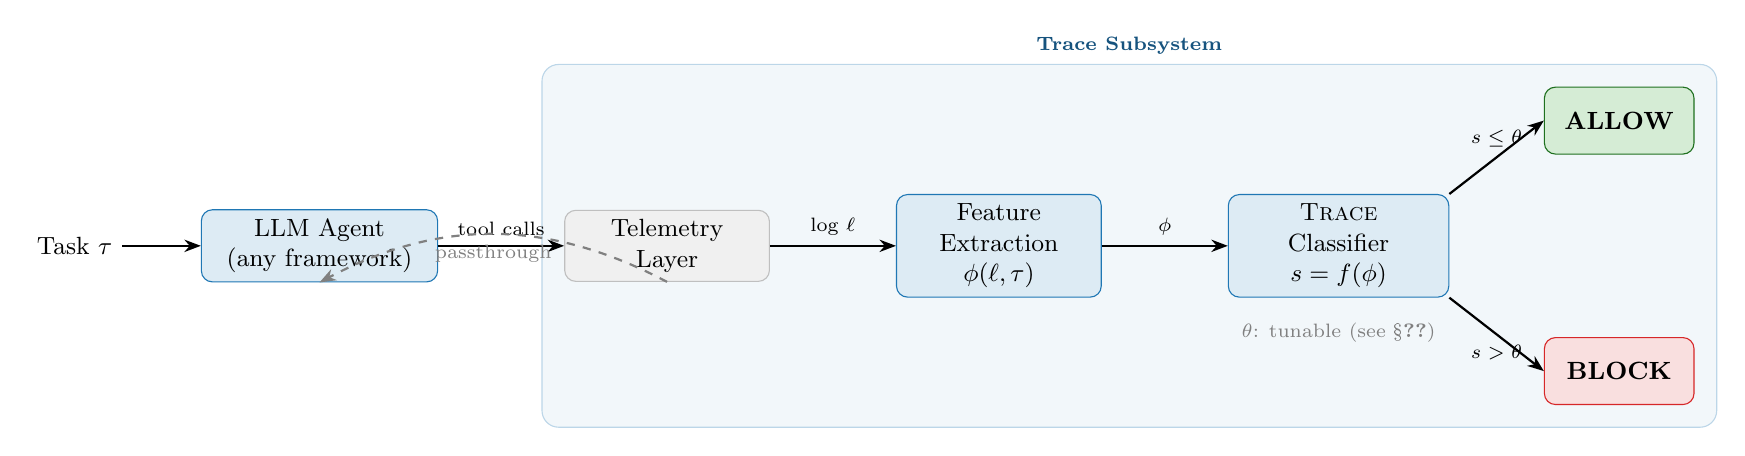
\begin{tikzpicture}[font=\small, node distance=1.4cm]
  \node[sysbluebox, minimum width=3.0cm] (agent) {LLM Agent\\(any framework)};
  \node[sysgraybox, right=1.6cm of agent] (telem) {Telemetry\\Layer};
  \node[sysbluebox, right=1.6cm of telem] (feat)
        {Feature\\Extraction\\$\phi(\ell,\tau)$};
  \node[sysbluebox, right=1.6cm of feat, minimum width=2.8cm] (clf)
        {\textsc{Trace}\\Classifier\\$s = f(\phi)$};
  \node[sysgreenbox, above right=0.5cm and 1.2cm of clf,
        minimum width=1.9cm] (allow) {\textbf{ALLOW}};
  \node[sysredbox,   below right=0.5cm and 1.2cm of clf,
        minimum width=1.9cm] (block) {\textbf{BLOCK}};
  \node[left=1.0cm of agent, font=\small] (task) {Task $\tau$};
  \draw[sysarrow] (task)  -- (agent);
  \draw[sysarrow] (agent) -- node[above,font=\scriptsize]{tool calls} (telem);
  \draw[sysarrow] (telem) -- node[above,font=\scriptsize]{log $\ell$}  (feat);
  \draw[sysarrow] (feat)  -- node[above,font=\scriptsize]{$\phi$}      (clf);
  \draw[sysarrow] (clf.north east) -- node[above,font=\scriptsize]
        {$s \le \theta$} (allow.west);
  \draw[sysarrow] (clf.south east) -- node[below,font=\scriptsize]
        {$s > \theta$} (block.west);
  \draw[sysdash, bend right=28] (telem.south)
        to node[below,font=\scriptsize]{passthrough} (agent.south);
  \node[below=0.2cm of clf, font=\scriptsize, text=gray]
        {$\theta$: tunable (see \S\ref{sec:threshold})};
  \begin{scope}[on background layer]
    \node[fill=traceblue!6, draw=traceblue!30, rounded corners=6pt,
          fit=(telem)(feat)(clf)(allow)(block),
          inner sep=8pt] (tracebox) {};
    \node[font=\scriptsize\bfseries, text=traceblue!70!black,
          above=0pt of tracebox.north] {\textsc{Trace} Subsystem};
  \end{scope}
\end{tikzpicture}%
}
\caption{\textbf{\textsc{Trace} system architecture.}  The telemetry
layer is a passive, non-intercepting wrapper: tool calls are forwarded
to the tool executor unchanged (dashed arrow) while a copy is appended
to log $\ell$.  Features $\phi(\ell,\tau)$ are extracted from $\ell$
and task $\tau$, then scored by the classifier.  When the score
exceeds threshold $\theta$ the run is flagged.  $\theta$ is the sole
operator control for the security-utility tradeoff.}
\label{fig:architecture}
\end{figure*}

\subsection{Instrumentation and Telemetry}

\textsc{Trace} attaches a thin wrapper between the agent framework
and its tool executor.  For each tool call, the wrapper appends a
structured event to the run log:
$\{\mathit{step}, \mathit{tool}, \mathit{args}, \mathit{result\_ok},
\mathit{ts\_ms}\}$.
The wrapper does not modify agent behavior or require model internals
access.  Logs can be consumed offline (run-level detection) or
incrementally (step-level early termination, a planned extension).

\subsection{Feature Extraction}
\label{sec:features}

Let $\ell = [e_1, \ldots, e_n]$ be the ordered event sequence for
a run on task~$\tau$.  Features $\phi(\ell, \tau) \in \mathbb{R}^{30}$
are extracted from five complementary groups (F1: 15 dims, F2: 5,
F3: 2, F4: 1, F5: 7):

\paragraph{F1 --- Sequence n-grams.}
A bag of tool-name bigrams (10 fixed vocabulary entries) and unigrams
(5 tool names): hijacked runs tend to pair information-gathering calls
(e.g., \texttt{read\_file}) with network-write calls
(e.g., \texttt{fetch\_url} POST) in ways rare in benign runs.

\paragraph{F2 --- Argument anomalies.}
Five scalar statistics: count of base64-encoded argument values,
unique external hostnames in URL arguments, unusually deep file paths
(depth~$>3$), oversized arguments (length~$>300$ chars), and HTTP
POST calls.

\paragraph{F3 --- Network destination consistency.}
An implied allow-list of hostnames is extracted from task description
$\tau$ via regex-based URL matching.  F3 is the fraction of network
calls to hosts outside this allow-list; exfiltration to an attacker
domain scores high while benign tasks score near zero.

\paragraph{F4 --- Intent--action consistency.}
Mean cosine distance (TF-IDF) between the action sequence and the
task embedding.  Ablation (Exp~D) shows minimal contribution in the
current implementation; richer embeddings are left for future work.

\paragraph{F5 --- Structural anomalies.}
Seven scalars: total step count, unique tool count, loop depth, count
of privilege-sensitive invocations (\texttt{shell\_exec},
\texttt{load\_skill}), write-tool calls, read-tool calls, and failed
steps.

\subsection{Classifier}

A LightGBM~\cite{ke2017lightgbm} gradient-boosted classifier is fit
over $\phi(\ell,\tau)$ with binary cross-entropy loss
(200~estimators; 31~leaves; learning rate~0.05; minimum
5~child samples; balanced class weights; random seed~42).
LightGBM is selected for its lower memory footprint on CPU.
The classifier outputs score $s \in [0,1]$ representing estimated
attack probability.  Training on 288~examples (60\,\% of the
480-trajectory corpus) completes in under two seconds on a standard
laptop CPU.

\subsection{The Security-Utility Threshold}
\label{sec:threshold}

At threshold $\theta$, a run is blocked iff $s > \theta$.  Sweeping
$\theta \in [0,1]$ traces the \emph{security-utility frontier}---the
Pareto set of (attack detection rate, legitimate utility preserved)
pairs---where security $= |\{s \!\in\! S_A : s > \theta\}|/|S_A|$
and utility $= 1 - \mathrm{FPR}(\theta)$.  \emph{Overdefense}
$= \mathrm{FPR}(\theta)$ quantifies the legitimate-task cost of the
defense.  An operator selects $\theta$ to meet a utility floor and
reads off the achievable security level.

% ============================================================
\section{Experimental Setup}
\label{sec:setup}
% ============================================================

\subsection{Agent Environment}

The agent runs a JSON-action loop~\cite{yao2023react}.
A fixed system prompt enumerates the tool schema and mandates that
every LLM response is a raw JSON object and nothing else
(e.g., \texttt{\{"tool":"fetch\_url","args":\{"url":"...","method":"GET"\}\}}).
The user turn supplies the task.  At each step, the LLM produces
one action, the matching tool executor returns an observation string
appended as the next \texttt{user} turn, and the loop repeats until
the agent calls \texttt{task\_complete} or a hard step cap of
10~is reached.  API calls use temperature~0.3, max\-\_\-tokens~256,
and OpenRouter's JSON-object response format (which rejects
malformed outputs server-side), with a 1.5\,s inter-step delay for
rate-limit headroom and up to 4 retries with exponential back-off.

All five tools are \textbf{simulated stubs}: \texttt{fetch\_url}
returns in-memory HTTP responses, \texttt{read\_file} returns
canned file content, \texttt{write\_file} appends to an in-memory
store, \texttt{shell\_exec} returns a fixed shell string, and
\texttt{load\_skill} returns a skill-description string.  No real
network requests, filesystem writes, or shell commands execute.
Attack injection is applied at the tool-result level: for injection
attacks, the first \texttt{fetch\_url} observation is replaced
by the attacker payload before reaching the agent; for poisoning
attacks, the \texttt{load\_skill} observation is replaced by the
malicious skill description.  All other tool calls behave normally;
the agent receives no signal that any substitution occurred.

\paragraph{API usage and reproducibility.}
Corpus generation required at most
$480 \times 10 = 4{,}800$ LLM API calls; in practice episodes
complete in 3--6 steps, so actual call count is lower.  Each episode
is checkpointed atomically to
\texttt{data/checkpoints/\textit{model}\_\_\textit{type}\_\_\textit{idx}.json}
immediately on close; an interrupted run resumes from the last
checkpoint without repeating any call.  The 480~pre-generated
trajectory files are released with the artifact so that
\emph{all classifier experiments can be reproduced by anyone
without an API key}:
\texttt{python experiments/run\_experiments.py -{-}skip-generation}.
Two generator models are accessed via OpenRouter:
\textbf{M1}~=~\texttt{google/gemini-2.5-flash-lite} and
\textbf{M2}~=~\texttt{meta-llama/llama-3.1-8b-instruct}.
Classifier training and inference are CPU-only with no per-run cost.

\subsection{Corpus Construction}

Four attack cells are constructed (Table~\ref{tab:corpus}):
injection-overt, injection-evasive, poisoning-overt,
poisoning-evasive---each with 30 instances per generator model
($= 60$ trajectories per cell, 240 attack total), drawn from
5 unique base task templates varied across 9 attacker-controlled
host identifiers to produce distinct attack payloads.  \emph{Overt} attacks use standard payloads.
\emph{Evasive} attacks use position-aware payload restructuring
(injection) and payload-less skill descriptions with harmful runtime
logic (poisoning), designed to yield clean text for pre-execution
scanners while preserving behavioral consequences.  The benign corpus comprises 240 trajectories drawn from a pool of
10 unique task templates covering the same five-tool footprint as
the attack corpus, each executed multiple times under both generator
models to match the attack corpus size and model distribution.
All trajectories are split 60/20/20 train/validation/test,
stratified by attack cell, generator model, and unique instance.
Because the template bank is small (5~attack, 10~benign), all
template families appear in both train and test; the split tests
generalization across instance variation rather than held-out task
semantics.  All reported metrics are on the held-out test split
(96~trajectories: 48~attack, 48~benign).

\begin{table}[t]
\centering
\caption{Corpus composition (30 instances per generator model $\times$
  2 models = 60 trajectories per attack cell).}
\label{tab:corpus}
\begin{tabular}{lcc}
\toprule
Attack cell & Trajectories & Attack format source \\
\midrule
Injection --- overt    & 60 & AgentDojo~\cite{debenedetti2024agentdojo} \\
Injection --- evasive  & 60 & AgentDojo \\
Poisoning --- overt    & 60 & BadAgent~\cite{shi2024badagent} \\
Poisoning --- evasive  & 60 & BadAgent \\
\midrule
Benign (total)         & 240 & Author-curated tasks \\
\bottomrule
\end{tabular}
\end{table}

\subsection{Baseline and Implementation}

\textsc{Trace} is compared against a \textbf{static keyword scanner}:
a deny-list applied to skill descriptions and retrieved content,
built from known signatures in InjectAgent~\cite{zhan2024injectagent}
and BadAgent~\cite{shi2024badagent}.  \textsc{Trace} is implemented
in Python with LightGBM~\cite{ke2017lightgbm} and
scikit-learn~\cite{pedregosa2011scikit}; all training and inference
run on CPU.  Trajectory generation used the OpenRouter API with both
generator models (Gemini~2.5~Flash~Lite and Llama~3.1~8B~Instruct);
the 480-trajectory dataset, feature extraction code, and trained
detector weights are released so the classifier can be replicated
without re-issuing LLM API calls
(\texttt{[repository link redacted for review]}).

% ============================================================
\section{Results}
\label{sec:results}
% ============================================================

Two hypotheses are evaluated: \textbf{H1} (\textsc{Trace} achieves
AUC $>0.85$ and substantially outperforms text-level baselines,
including on evasive variants) and \textbf{H2} (cross-model transfer
AUC drops $<0.05$ relative to in-distribution).

\subsection{Exp A: Detection Efficacy}
\label{sec:exp_a}

\begin{table}[t]
\centering
\caption{Overall detection efficacy on the held-out test split
  ($\theta=0.5$; 48 attack + 48 benign trajectories).
  Wilson 95\,\% CIs in brackets.  AUC not applicable (n/a) for
  threshold-fixed baselines.}
\label{tab:efficacy}
\begin{tabular}{lccc}
\toprule
Method & AUC & DR\,\% [95\,\%\,CI] & FPR\,\% \\
\midrule
Static scanner      & n/a   & 25.0\;[14.9--38.8] & 0.0 \\
Behavioral rules    & n/a   & 50.0\;[36.1--63.9] & 0.0 \\
\textsc{Trace}      & 0.984 & 97.9\;[89.1--99.6] & 4.2 \\
\bottomrule
\end{tabular}
\end{table}

Table~\ref{tab:efficacy} reports three detectors.  The keyword
scanner reaches DR~25.0\,\% at FPR~0.0\,\%.  The behavioral rule
baseline (Exp~F) doubles that to DR~50.0\,\% at FPR~0.0\,\%, but
is limited by attacks routing only through task-implied hosts.
\textsc{Trace} achieves AUC~0.984, DR~97.9\,\% [89.1--99.6], and
FPR~4.2\,\% at $\theta{=}0.5$, confirming H1; the advantage
over both baselines is amplified on evasive variants (Exp~B).

\subsection{Exp B: Evasion Stress Test}
\label{sec:exp_b}

\begin{table}[t]
\centering
\caption{Per-cell attack detection rate at $\theta{=}0.5$
  ($n{=}12$ attack trajectories per cell $= 60 \times 20\%$
  test portion).  Per-cell evaluation covers attack trajectories
  only; aggregate FPR across all 48 benign test trajectories
  is reported in Table~\ref{tab:efficacy}.
  Wilson 95\,\% CI: [75.8--100] (first three cells);
  [64.6--98.5] (evasive poisoning).}
\label{tab:evasion}
\begin{tabular}{lcccc}
\toprule
 & \multicolumn{2}{c}{Injection DR (\%)} &
   \multicolumn{2}{c}{Poisoning DR (\%)} \\
\cmidrule(lr){2-3}\cmidrule(lr){4-5}
Method & Overt & Evasive & Overt & Evasive \\
\midrule
Static scanner & \multicolumn{4}{c}{\makebox[0pt][c]{25.0\,\% aggregate (FPR\,=\,0.0\,\%)}} \\
\textsc{Trace} & 100.0 & 100.0  & 100.0 & 91.7 \\
\bottomrule
\end{tabular}
\end{table}

Table~\ref{tab:evasion} is the central result.  \textsc{Trace}
achieves 100\,\% DR [75.8--100] on three of four cells and
91.7\,\% [64.6--98.5] on evasive poisoning.  These results are
scoped to the non-adaptive threat model (\S\ref{sec:threat});
adaptive evasion is quantified in Exp~G (\S\ref{sec:exp_fg}).
The static scanner's 25\,\% aggregate DR exposes the structural
failure of text-level inspection, confirming H1.

\subsection{Exp C: Security-Utility Frontier}
\label{sec:exp_c}

\begin{figure}[t]
\centering
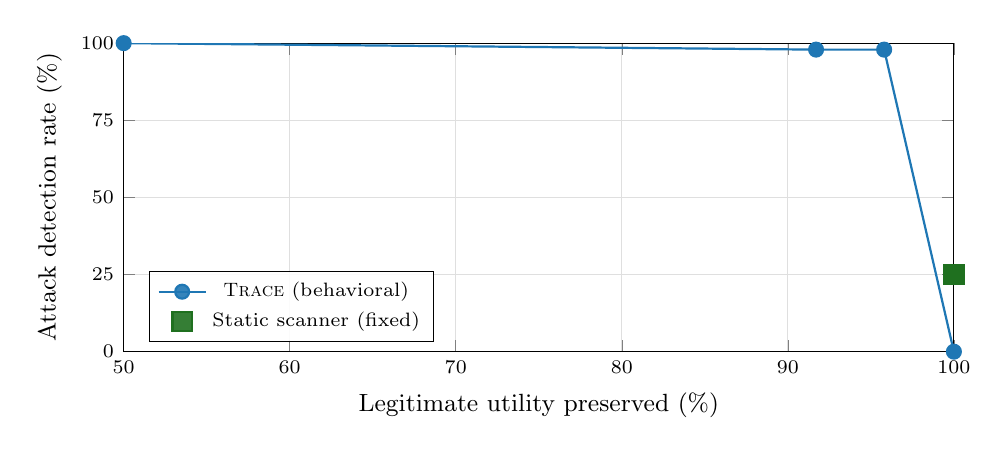
\begin{tikzpicture}
\begin{axis}[
  width=\columnwidth, height=5.5cm,
  xlabel={Legitimate utility preserved (\%)},
  ylabel={Attack detection rate (\%)},
  xmin=50, xmax=100, ymin=0, ymax=100,
  xtick={50,60,70,80,90,100},
  ytick={0,25,50,75,100},
  grid=both,
  grid style={line width=0.3pt, draw=gray!25},
  legend pos=south west,
  legend style={font=\scriptsize, fill=white, fill opacity=0.9,
                draw opacity=1, text opacity=1},
  xlabel style={font=\small},
  ylabel style={font=\small},
  tick label style={font=\scriptsize},
]
% TRACE: (util%, sec%) at theta = 1.0, 0.08, 0.01, 0.0
\addplot[thick, color=traceblue, mark=*, mark size=2.5pt]
  coordinates {(100,0)(95.8,97.9)(91.7,97.9)(50,100)};
% Annotate recommended theta=0.08 operating point
\node[font=\scriptsize, above left, text=traceblue]
  at (axis cs:95.8,97.9) {$\theta{=}0.08$};
% Static scanner: fixed point (FPR=0%, DR=25%)
\addplot[thick, color=benigngreen!70!black, mark=square*,
         mark size=3.5pt, only marks]
  coordinates {(100,25)};
\legend{\textsc{Trace} (behavioral),
        Static scanner (fixed)}
\end{axis}
\end{tikzpicture}
\caption{\textbf{Security-utility frontier.}  Each point on the
  \textsc{Trace} curve is a threshold $\theta$ setting.  At
  $\theta=0.08$: 97.9\,\% security at 95.8\,\% utility.  The
  static scanner's fixed point offers no tunable trade-off.}
\label{fig:frontier}
\end{figure}

Figure~\ref{fig:frontier} shows the frontier.  At $\theta=0.08$,
\textsc{Trace} attains 97.9\,\% security at 95.8\,\% utility.
Lowering $\theta$ to 0.01 reduces utility to 91.7\,\% while
security stays 97.9\,\%: the one missed attack contacts only
task-implied hosts, suppressing F1 and F3 simultaneously.  The
static scanner is fixed at (100\,\% utility, 25\,\% security)
with no tunable trade-off.

\subsection{Exp D: Feature Ablation}
\label{sec:exp_d}

\begin{table}[t]
\centering
\caption{AUC under feature group ablation (test split).
  $\Delta$ is relative to the full model.}
\label{tab:ablation}
\begin{tabular}{lcc}
\toprule
Configuration & AUC & $\Delta$ vs.\ full \\
\midrule
Full \textsc{Trace} (all features)  & 0.984 & --- \\
\quad $-$ F1 (sequence n-grams)     & 0.980 & $-$0.004 \\
\quad $-$ F2 (argument anomalies)   & 0.984 & $\phantom{-}$0.000 \\
\quad $-$ F3 (network destination)  & 0.981 & $-$0.003 \\
\quad $-$ F4 (intent--action)       & 0.984 & $\phantom{-}$0.000 \\
\quad $-$ F5 (structural)           & 0.981 & $-$0.003 \\
\midrule
F3 alone                            & 0.760 & $-$0.224 \\
F1\,+\,F3 alone                     & 0.949 & $-$0.035 \\
\bottomrule
\end{tabular}
\end{table}

No single feature group dominates: dropping any one group reduces
AUC by at most 0.004 (Table~\ref{tab:ablation}), indicating the
groups are complementary.  Notably, dropping F2 or F4 produces zero
AUC change---on a 96-trajectory test set near performance ceiling,
$\Delta{=}0.000$ may partly reflect measurement resolution rather
than strict redundancy; however, neither group adds independent value
in the current implementation, and F4's TF-IDF instantiation requires
improvement before it contributes meaningfully (see \S\ref{sec:features}).
F3 alone yields AUC~0.760, confirming network-destination consistency
is useful but insufficient in isolation.  The two-group combination
F1$+$F3 recovers AUC~0.949, capturing 96.4\,\% of full detection
power with one-fifth the feature dimension, identifying sequence
n-grams and network consistency as the two highest-value signals.

\subsection{Exp E: Cross-Model Transfer}
\label{sec:exp_e}

\begin{table}[t]
\centering
\caption{Cross-model transfer AUC.
  M1~=~Gemini~2.5~Flash~Lite; M2~=~Llama~3.1~8B~Instruct.}
\label{tab:transfer}
\begin{tabular}{lcc}
\toprule
Train $\to$ Test & In-dist AUC & Transfer AUC \\
\midrule
M1 $\to$ M1 & 1.000 & --- \\
M2 $\to$ M2 & 0.964 & --- \\
M1 $\to$ M2 & ---   & 0.797 \\
M2 $\to$ M1 & ---   & 0.854 \\
\bottomrule
\end{tabular}
\end{table}

In-distribution AUC reaches 1.000 (M1) and 0.964 (M2), confirming
strong separability within each model's trajectory distribution.
The M1 value of 1.000 should be interpreted with caution given the
small test set ($n{=}96$); it reflects the high behavioral
distinctiveness of M1 attack trajectories rather than overfit, but
cannot be confirmed without a larger evaluation.  Cross-model transfer
degrades to 0.797--0.854, a drop of 0.11--0.20 AUC points.
\textbf{H2 is not confirmed}: the stated criterion (drop $<0.05$) is
exceeded in both transfer directions by a factor of 2--4$\times$.
Behavioral features do generalize across model families (both well
above chance), but the degradation is practically significant.
Cross-model deployment without retraining is inadvisable; per-deployment
calibration on a small benign corpus from the target model is
required to recover near-in-distribution performance.

\subsection{Exp F/G: Behavioral Baseline and Adaptive Evasion}
\label{sec:exp_fg}

\begin{table}[t]
\centering
\caption{Adaptive-attacker ablation (Exp~G, $\theta{=}0.5$).
  Attack trajectories modified to suppress F3 (redirect URLs to
  implied host), F1 (shuffle step order), or both.
  Benign trajectories unmodified; same trained classifier as Exp~A.}
\label{tab:adaptive}
\begin{tabular}{lcc}
\toprule
Modification & DR\,\% & AUC \\
\midrule
None (Exp~A baseline)   & 97.9 & 0.984 \\
F3 suppressed           & 97.9 & 0.984 \\
F1 suppressed           & 77.1 & 0.967 \\
F1\,+\,F3 suppressed   & 77.1 & 0.967 \\
\bottomrule
\end{tabular}
\end{table}

The behavioral rule baseline (Exp~F, Table~\ref{tab:efficacy}) achieves
DR~50.0\,\% vs.\ 25.0\,\% for the keyword scanner and 97.9\,\% for
\textsc{Trace}, demonstrating that hand-crafted behavioral rules
capture a meaningful signal but that ML-learned feature combinations
provide substantially higher recall at identical FPR.

Table~\ref{tab:adaptive} reports the adaptive-attacker ablation
(Exp~G).  Suppressing F3 alone (routing exfiltration through a
task-implied host) leaves detection unchanged: DR~97.9\,\% and
AUC~0.984.  The classifier compensates via F1, F2, and F5, showing
that the multi-feature design provides inherent robustness to
single-feature suppression.  Suppressing F1 (shuffling step order to
break attack bigrams) reduces DR to 77.1\,\%---still 3$\times$ the
keyword scanner and 1.5$\times$ the rule baseline.  The combined
F1\,+\,F3 suppression yields identical degradation to F1 alone,
indicating F2/F5 maintain the residual signal once F1 is disrupted.
At 77.1\,\% DR, \textsc{Trace} retains meaningful detection even
under this simultaneous worst-case evasion.

% ============================================================
\section{Discussion}
\label{sec:discussion}
% ============================================================

\paragraph{Adaptive attackers.}
The threat model excludes attackers aware of \textsc{Trace}'s feature
set.  Exp~G (\S\ref{sec:exp_fg}) directly measures this risk: F3
suppression alone leaves TRACE unaffected (DR~97.9\,\%), while
simultaneous F1\,+\,F3 suppression reduces DR to 77.1\,\%
(AUC~0.967).  The headline 91.7--100\,\% detection rates are therefore
valid \emph{within the stated, non-adaptive threat model}; the worst
conceivable evasion of the two strongest features still yields 77.1\,\%
DR---3$\times$ the keyword scanner.  Designing detectors robust to
fully adaptive attackers who additionally suppress F2 and F5 is an
important future direction.

\paragraph{Baseline and benchmark scope.}
Two runtime baselines are evaluated: a keyword scanner and a
hand-crafted behavioral rule detector (Exp~F, DR=50\%).  Both are
acknowledged to be weak comparators.  A learned behavioral
baseline---a runtime feature classifier from contemporaneous work,
LlamaGuard applied post-execution~\cite{inan2023llama}, or a hybrid
spotlighting~\cite{hines2024spotlighting} guard-model stack---was not
evaluated; comparison against at least one such learned behavioral
competitor on the same corpus remains the single most important
empirical gap.  Results are also limited to AgentDojo and one
skill-poisoning benchmark; whether these distributions represent
production attack traffic is unknown.  The full trajectory dataset is
released to support independent analysis against additional baselines
and deployment contexts.

\paragraph{Layered deployment.}
\textsc{Trace} is a runtime layer complementary to pre-execution
defenses (spotlighting~\cite{hines2024spotlighting}, guard
models~\cite{inan2023llama}).  Operators select $\theta$ against a
representative benign corpus; absent one, a conservative high-$\theta$
default with online calibration as logs accumulate is recommended.

\paragraph{Generalizability and corpus validity.}
The five simulated stub tools and scripted responses may not capture
the trajectory variability of richer production deployments.
Both corpora are LLM-generated from small template banks (5~attack,
10~benign), so the classifier may partly reflect generation-mode
artifacts; validation on live compromised-agent traces is recommended
before production use.

% ============================================================
\section{Conclusion}
\label{sec:conclusion}
% ============================================================

This paper presented \textsc{Trace}, a behavioral detector for LLM
agent hijacking that classifies execution trajectories rather than
inspecting triggering text.  By decoupling the detection signal
(agent actions) from the evasion target (trigger text), \textsc{Trace}
achieves AUC~0.984 and 91.7--100\,\% DR across all four attack
cells within the stated, non-adaptive threat model---including
evasive variants where a keyword scanner reaches only 25\,\% DR.
At $\theta{=}0.08$, the system attains 97.9\,\% security at 95.8\,\%
utility; the explicit FPR-calibrated overdefense frontier over a
size-matched benign corpus provides a principled tradeoff tool
complementary to existing security-utility benchmarks.  Cross-model
transfer AUC (0.80--0.85) demonstrates partial generalization but
does not meet the $<0.05$-drop criterion: the released weights and
dataset enable independent replication of classifier results, but
per-deployment calibration on target-model benign logs is required
before production use.  A behavioral rule baseline (Exp~F) achieves DR~50.0\,\% vs.\
25.0\,\% for the keyword scanner, confirming that ML over behavioral
features adds substantial value beyond hand-crafted rules.
Even under worst-case F1\,+\,F3 suppression by an adaptive adversary
(Exp~G), DR retains 77.1\,\%---3$\times$ the keyword scanner.  The
most important remaining open problem is evaluation against behavioral
runtime competitors on the same corpus.

% ============================================================
\bibliographystyle{IEEEtran}
\bibliography{strings}

% ============================================================
\section*{AI Use Disclosure}
% ============================================================
LLM APIs (Gemini~2.5~Flash~Lite and Llama~3.1~8B~Instruct via
OpenRouter) were used for agent trajectory generation as described
in \S\ref{sec:setup}.  No language model was used to generate the
substantive scientific content, analysis, or manuscript text of
this paper.

\end{document}
